\documentclass{article}
\usepackage[utf8]{inputenc}
\textheight = 25cm 
\textwidth = 15cm
\topmargin = -2.5cm 
\oddsidemargin = 1.5cm
\usepackage{float}
\usepackage{graphicx}
\graphicspath{{./images/}}

\usepackage{amsmath}
\usepackage{mathtools, xparse}
\usepackage[shortlabels]{enumitem}
\usepackage[most]{tcolorbox}
\usepackage{adjustbox}
\usepackage{bm} 

\DeclarePairedDelimiter{\norm}{\lVert}{\rVert}

\title{Parcial II Mecánica Analítica}
\author{Cerritos Lira Carlos}
\date{8 de Junio del 2020}

\begin{document}
\maketitle
\section*{Problemas}
\section*{1.-}
Una partícula positiva de carga $e$ (fig. 6-16) se mueve en el campo eléctrico central
\[ \bm{E} = -\frac{\alpha}{\rho} \bm{e}_{\rho} \]
que hay entre las placas de un condensador cilíndrico, y en un campo magnético uniforme:
\[ \bm{B} = B\bm{k} \]
paralelo al eje del condensador.
\begin{enumerate}[a)]
    \item Establecer las ecuaciones de movimiento de la partícula en coordenadas cilíndricas.
    \item Demostrar que la ecuación de movimiento, en función de la variable anular $\phi$, que es 
    una coordenada que se puede no considerar, se resuelve fácilmente y da como integral de movimiento 
    \[ m\rho^2\dot{\phi} + \frac{1}{2}e\rho^2B = h = constante \]
    \item Demuestrar que, utilizando el resultado hallado en $b)$, la ecuación radial se puede 
    reducir a una ecuación de movimiento unidimensional, que nos dará una segunda integral del movimiento 
    que expresa la conservación de la energía total. 
    \item Si la partícula es emitida del cilindro interior con una velocidad:
    \[ \bm{v}_0 = v_0\bm{e}_\rho \]
    ¿cuál debe ser el valor mínimo de $v_0$ para que la partícula llegue al otro cilindro cuyo radio es $R_2$.
    [Sugerencia: el valor mínimo de $v_0$ se obtendrá cuando $R_2$ sea un punto de retorno]
\end{enumerate}
\begin{figure}[H]
    \centering
    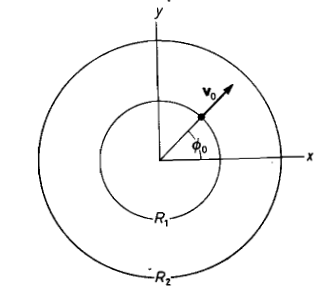
\includegraphics[scale=0.6]{images/p1_diagram.png}
    \caption{Condensador cilíndrico}
\end{figure}
\begin{tcolorbox}[breakable]
    \subsubsection*{a)}
    Recordamos que en coordenadas cilíndricas:
    \begin{align*}
        \bm{r} &= \rho cos\phi \bm{i} + \rho sin\phi\bm{j} + z\bm{k} \\
        \bm{v} 
        &=(\dot{\rho} cos\phi - \rho \dot{\phi}sin\phi) \bm{i} 
        + (\dot{\rho}sin\phi + \rho \dot{\phi}cos\phi) \bm{j} 
        + \dot{z}\bm{k} \\
        v^2 &= \dot{\rho}^2 + \rho^2\dot{\phi}^2 + \dot{z}^2 \\ 
        \bm{e}_\rho &= cos\phi \bm{i} + sin\phi \bm{j} 
    \end{align*}
    El campo eléctrico y magnético son de la forma:
    \begin{align*}
        \bm{E} &= -\nabla \Phi = -\bm{\nabla} \alpha ln(\rho) \\ 
        \bm{B} &= \nabla \times \bm{A} 
    \end{align*}
    en este caso $\bm{A}$ está dado por:
    \begin{align*}
        \bm{A} 
        &= -\frac{1}{2}(\bm{r} \times \bm{B}) \\
        &= -\frac{1}{2}(\bm{r} \times B\bm{k}) \\
        &= -\frac{1}{2}B\rho(sin\phi \bm{i} - cos\phi \bm{j}) \\
        \bm{v} \cdot \bm{A} 
        &= -\frac{1}{2}B\rho 
        \bigg[ sin\phi (\dot{\rho} cos\phi - \rho \dot{\phi}sin\phi) 
        -cos\phi (\dot{\rho}sin\phi + \rho \dot{\phi}cos\phi) \bigg] \\
        &= \frac{1}{2}B\rho^2 \dot{\phi}(cos\phi^2 + sin\phi^2) \\
        &= \frac{1}{2}B\rho^2 \dot{\phi} 
    \end{align*}
    de donde obtenemos:
    \begin{align*}
        L 
        &= T - U + e\bm{v} \cdot \bm{A} \\
        &= \frac{1}{2}m(\dot{\rho}^2 + \rho^2\dot{\phi}^2 + z^2) - e\alpha ln(\rho) + \frac{1}{2}eB\rho^2 \dot{\phi}
    \end{align*}
    recordamos que se satisface la relación:
    \begin{align*}
        \frac{\partial L}{\partial q_i} - \frac{d}{dt}\frac{\partial L}{\partial \dot{q}_i} &= 0
    \end{align*}
    aplicado a $\phi$ obtenemos:
    \begin{align*}
        \frac{\partial L}{\partial \phi} - \frac{d}{dt}\frac{\partial L}{\partial \dot{\phi}} &= 0 \\
        \frac{d}{dt}(m\rho^2\dot{\phi} + \frac{1}{2}eB\rho^2) &= 0
     \end{align*}
     aplicado a $\rho$ obtenemos:
    \begin{align*}
        \frac{\partial L}{\partial \rho} - \frac{d}{dt}\frac{\partial L}{\partial \dot{\rho}} &= 0 \\
        m\rho \dot{\phi}^2 - e\alpha \frac{1}{\rho} + eB\rho \dot{\phi} - \frac{d}{dt}(m\dot{\rho}) &= 0 \\
        m\rho \dot{\phi}^2 - e\alpha \frac{1}{\rho} + eB\rho \dot{\phi} - m\ddot{\rho} &= 0 
    \end{align*}
    aplicado a $z$ obtenemos:
    \begin{align*}
        mz &= 0
    \end{align*}
    \subsubsection*{b)}
    De la ecuación de movimiento obtenida en $a)$, para $\phi$ se tiene:
    \begin{align*}
        \frac{d}{dt}(m\rho^2\dot{\phi} + \frac{1}{2}eB\rho^2) &= 0 \\
        m\rho^2\dot{\phi} + \frac{1}{2}e\rho^2B &= h
    \end{align*}
    \subsubsection*{c)}
    De la ecuación de movimiento obtenida en $a)$, para $\rho$ se tiene:
    \begin{align*}
        m\rho \dot{\phi}^2 - e\alpha \frac{1}{\rho} + eB\rho \dot{\phi} - m\ddot{\rho} &= 0 \\
        h\rho \dot{\phi} +  \frac{1}{2}eB\rho \dot{\phi} - e\alpha \frac{1}{\rho}  - m\ddot{\rho} &= 0
    \end{align*}
    donde se observa obtuvimos una ecuación unidimensional para $\rho$
    \subsubsection*{d)}
    Calculamos $H = p_i\dot{q}_i - L$:
    \begin{align*}
        H 
        &= p_i\dot{q}_i - L \\
        &= 
    \end{align*}

\end{tcolorbox}
\newpage
\section*{2.-}
\begin{enumerate}[a)]
    \item Establezca las ecuaciones de Euler-Lagrange para la máquina de Atwood doble, 
    fig.2, desprecie el efecto de las poleas en el movimiento, lidie con las constricciones del problema usando multiplicadores 
    de Lagrange en las ecuaciones de movimiento.
    \begin{figure}[H]
        \centering
        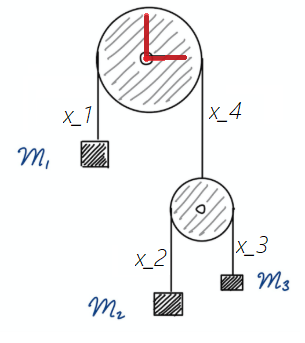
\includegraphics[scale=0.7]{p2_atwood.png}
        \caption{Máquina de Atwood doble}
    \end{figure}
    \item Encuentre las tensiones en las cuerdas y las aceleraciones de las masas de forma explicita, expresandolas(tanto las tensiones como las aceleraciones)
    solo en términos de $g$ y las masas $(m_1,m_2,m_3)$. \\
    \textit{Hint:1 Derive dos veces las constricciones respecto al tiempo, esto podría llevar a ecuaciones que pueden facilitar 
    el álgebra para despejar los valores que se pdien.} \\
    \textit{Hint 2: Las tensiones de las cuerdas son las fuerzas de constricción.} 
    \[ T_i = Q_i = \sum_k \lambda_k \frac{\partial \phi_k}{\partial q_i} \]
\end{enumerate}
\begin{tcolorbox}[breakable]
    \subsubsection*{a)}
    Supongamos que las cuerdas son de longitud $l_1$ y $l_2$ respectivamente, usando las coordenadas generalizadas
    descritas en la figura 2 obtenemos:
    \begin{align*}
        \bm{r}_1 &= -x_1 \bm{j} \\
        \bm{r}_2 &= -(x_4+x_2) \bm{j} \\
        \bm{r}_3 &= -(x_4+x_3) \bm{j}
    \end{align*}
    tenemos las constricciones:
    \begin{align*}
        \phi_1(x_1,x_2,x_3,x_4) &= x_1 + x_4 - l_1 = 0 \\
        \phi_2(x_1,x_2,x_3,x_4) &= x_2 + x_3 - l_2 = 0 
    \end{align*}
    bajo estas coordenadadas se tiene:
    \begin{align*}
        T
        &= T_1 + T_2 + T_3 \\
        &=\frac{1}{2}m_1\dot{x}_1^2 
        + \frac{1}{2}m_2(\dot{x}_4 + \dot{x}_2)^2
        + \frac{1}{2}m_3(\dot{x}_4 + \dot{x}_3)^2 \\
        U 
        &= U_1 + U_2 + U_3 \\
        &= -m_1gx_1-m_2g(x_4+x_2)-m_3g(x_4+x_3)
    \end{align*}
    usando las ecuaciones de Lagrange obtenemos:
    \begin{align*}
        \frac{\partial L}{\partial q_i} 
        -\frac{d}{dt}\frac{\partial L}{\partial \dot{q}_i} 
        + \sum_k \lambda_k \frac{\partial \phi_k}{\partial q_i}
        &= 0  
    \end{align*}
    para $x_1$ tenemos:
    \begin{align*}
        \frac{\partial L}{\partial x_1} 
        -\frac{d}{dt}\frac{\partial L}{\partial \dot{x}_1} 
        + \sum_k \lambda_k \frac{\partial \phi_k}{\partial x_1}
        &= 0  \\
        m_1g - m_1\ddot{x}_1 + \lambda_1 &= 0 \\
        \ddot{x}_1 &= \frac{\lambda_1}{m_1} + g
    \end{align*}
    para $x_4$ tenemos:
    \begin{align*}
        \frac{\partial L}{\partial x_4} 
        -\frac{d}{dt}\frac{\partial L}{\partial \dot{x}_4} 
        + \sum_k \lambda_k \frac{\partial \phi_k}{\partial x_4}
        &= 0  \\
        m_2g+m_3g - m_2(\ddot{x}_4+\ddot{x}_2) - m_3(\ddot{x}_4+\ddot{x}_3) + \lambda_1 &= 0
    \end{align*}
    para $x_2$ tenemos:
    \begin{align*}
        \frac{\partial L}{\partial x_2} 
        -\frac{d}{dt}\frac{\partial L}{\partial \dot{x}_2} 
        + \sum_k \lambda_k \frac{\partial \phi_k}{\partial x_2}
        &= 0  \\
        m_2g-m_2(\ddot{x}_4+\ddot{x}_2) + \lambda_2 &= 0 \\
        \ddot{x}_4+\ddot{x}_2 &= \frac{\lambda_2}{m_2} + g
    \end{align*}
    para $x_3$ tenemos:
    \begin{align*}
        \frac{\partial L}{\partial x_3} 
        -\frac{d}{dt}\frac{\partial L}{\partial \dot{x}_3} 
        + \sum_k \lambda_k \frac{\partial \phi_k}{\partial x_3}
        &= 0  \\
        m_3g - m_3(\ddot{x}_4+\ddot{x}_3) + \lambda_1 &= 0 \\
        \ddot{x}_4+ \ddot{x}_3 &= \frac{\lambda_2}{m_3}+g
    \end{align*}
    usando la relación para $x_4,x_2$ y $x_3$ se obtiene una relación entre $\lambda_1$ y $\lambda_2$:
    \begin{align*}
        \lambda_1 
        &= m_2(\ddot{x}_4+\ddot{x}_2) + m_3(\ddot{x}_4+\ddot{x}_3) - g(m_2+m_3) \\
        &= \lambda_2 + \lambda_2 + g(m_2+m_3) - g(m_2+m_3) \\
        &= 2\lambda_2 
    \end{align*}
    de las ecuaciones de constricción tenemos además:
    \begin{align*}
        \ddot{x_1}+\ddot{x_4} &= 0 \\
        \ddot{x_2}+\ddot{x_3} &= 0 \\ 
        \ddot{x_1}-\ddot{x_2} &= -(\ddot{x_4}+\ddot{x}_2) = -\tfrac{\lambda_2}{m_2}-g \\
        \ddot{x_1}+\ddot{x_2} &= -(\ddot{x}_4+\ddot{x}_3) = -\tfrac{\lambda_2}{m_3}-g 
    \end{align*}
    despejamos $x_1$ y usamos la relación obtenida para esta coordenada anteriormente:
    \begin{align*}
        2\ddot{x}_1 &= -\tfrac{\lambda_2}{m_2}-\tfrac{\lambda_2}{m_3}-2g \\
        2(\tfrac{\lambda_1}{m_1}+g) &= -\tfrac{\lambda_2}{m_2}-\tfrac{\lambda_2}{m_3}-2g \\
        4g &= -\lambda_2(\tfrac{4}{m_1}+\tfrac{1}{m_2}+\tfrac{1}{m_3}) \\
        \lambda_2 &= \frac{4g}{\tfrac{4}{m_1}+\tfrac{1}{m_2}+\tfrac{1}{m_2}} 
    \end{align*} 
    \subsubsection*{b)}
    La tensión para la cada cuerdas es:
    \begin{align*}
        T_1 &= \sum_k \lambda_k \frac{\partial \phi_k}{\partial x_1} = \lambda_1 = 2\lambda_2 \\
        T_2 &= \sum_k \lambda_k \frac{\partial \phi_k}{\partial x_2} = \lambda_2
    \end{align*}

\end{tcolorbox}
\newpage
\section*{3.-}
En la fig.3 se muestra un regulador centrífugo de una máquina de vapor. Dos bolas, cada una de masa $m$, están unidas por cuatro brazos articulados, 
cada uno de longitud $l$, a unos manguitos colocados sobre un eje redondo vertical. El manguito superior está sujeto al eje; el inferior, de masa $M$, 
se puede deslizar libremente hacia arriba o hacia abajo a lo largo del eje, amedida que las bolas se alejan o se acercan al mismo. 
El sistema del eje y las bolas giran con velocidad angular constante $w$.
\begin{figure}[H]
    \centering
    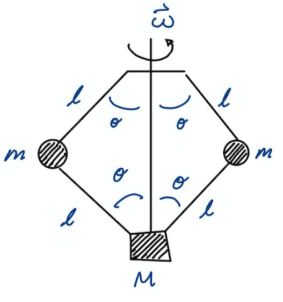
\includegraphics[scale=1]{p3_system.png}
    \caption{Regulador centrífugo}
\end{figure}

\begin{enumerate}[a)]
    \item Escriba el lagrangiano del sistema.
    \item Obtenga las ecuaciones de movimiento, despreciando el pesos de los brazos y el eje. Estúdiese el movimiento por el método de la energía.
    \item Determínese la altura, $z$ del magnuito inferior por encima de su posición más baja, en función de $w$ para la rotación estacionaria de las bolas 
    y determínese la frecuencia de las pequeñas oscilaciones de $z$ a un lado y otro de su valor estacionario.
\end{enumerate}
\begin{tcolorbox}[breakable]
    \subsubsection*{a)}
    Usaremos las coordenadada generalizada $\theta$, se tiene:
    \begin{align*}
        \bm{r}_1 &= l \sin\theta \sin wt\bm{i} + l\sin\theta \cos wt \bm{j} - l\cos\theta \bm{k}\\
        \bm{\dot{r}}_1 
        &=(l\dot{\theta} \cos\theta \sin wt + lw \sin\theta \cos wt) \bm{i} 
        + (l\dot{\theta} \cos\theta \cos wt - lw\sin\theta \sin wt)\bm{j}
        - l\dot{\theta} \sin\theta \bm{k} \\
        \dot{r}_1^2 
        &=l^2\dot{\theta}^2cos^2\theta + l^2\dot{\theta}\sin^2\theta 
        = l^2\dot{\theta}^2 + l^2w^2\sin^2\theta \\ 
        \bm{r}_2 &= -2l \cos \theta \bm{k} \\
        \dot{r}_2^2 &= 4l^2\dot{\theta}^2\sin^2\theta
    \end{align*}
    de donde obtenemos:
    \begin{align*}
        T 
        &= 2T_1 + T_2 \\
        &= m(l^2\dot{\theta}^2+l^2w^2sin^2\theta) + 2Ml^2\dot{\theta}^2 \sin^2\theta \\
        U
        &= -2mglcos\theta - 2Mglcos\theta
    \end{align*}
    cálculamos el Lagrangiano por definición:
    \begin{align*}
        L 
        &= T-U \\
        &= m(l^2\dot{\theta}^2+l^2w^2sin^2\theta) + 2Ml^2\dot{\theta}^2 \sin^2\theta + 2gl(m\cos\theta + M\cos\theta)
    \end{align*}
    \subsubsection*{b)}
    Para $\theta$ obtenemos:
    \begin{align*}    
        \frac{\partial L}{\partial \theta} 
        &=2ml^2w^2\sin\theta \cos\theta 
        + 4Ml^2\dot{\theta}^2\sin\theta \cos\theta 
        -2glsin\theta(m+M) \\
        \frac{d}{dt}\frac{\partial L}{\partial \dot{\theta}} 
        &= \frac{d}{dt}(2ml^2\dot{\theta} + 4Ml^2\dot{\theta}\sin^2\theta) 
        = 2ml^2\ddot{\theta} + 4Ml^2(\ddot{\theta}\sin^2\theta + 2\dot{\theta}^2\sin\theta \cos\theta)
    \end{align*}
    Utilizando la relación:
    \begin{align*}
        \frac{\partial L}{\partial \theta} - \frac{d}{dt}\frac{\partial L}{\partial \dot{\theta}} &= 0 \\
        2ml^2w^2\sin\theta \cos\theta 
        -4Ml^2\dot{\theta}^2\sin\theta \cos\theta 
        -2glsin\theta(m+M) 
        -2l^2\ddot{\theta}(m + 2M\sin^2\theta)  
        &= 0
    \end{align*}
    \subsubsection*{c)}
    En una rotación estaconaria se tiene $\dot{\theta} = 0, \ddot{\theta} = 0$, usando la ecuación de $b)$ para $\theta$ obtenemos:
    \begin{align*}
        2ml^2w^2\sin\theta \cos\theta 
        -2gl\sin\theta(m+M)   
        &= 0 \\
        2ml^2w^2\sin\theta \cos\theta
        &= 2gl\sin\theta(m+M) \\
        cos\theta &= \tfrac{g}{lw^2}(1+\tfrac{M}{m})
    \end{align*} 
    $z$ se pude obtener como:
    \begin{align*}
        z 
        &= 2l(1-cos\theta) \\
        &= 2l[1-\tfrac{g}{lw^2}(1+\tfrac{M}{m})]
    \end{align*}
    ahora bien, si tomamos $w=0,M=0$, de la ecacuión para $\theta$ obtenida en $b)$ tenemos:
    \begin{align*}
        2glmsin\theta 
        +2ml^2\ddot{\theta}  
        &= 0 \\
        \ddot{\theta} + \frac{g}{l}sin\theta &= 0
    \end{align*} 

\end{tcolorbox}

\end{document}
